\documentclass{article}
\usepackage[utf8]{inputenc}
\usepackage{imakeidx}
\usepackage{amsmath}
\usepackage[italian]{babel}
\usepackage{graphicx}
\usepackage[T1]{fontenc}
\usepackage[margin=1in]{geometry}
\usepackage{bm}
\makeindex
\usepackage{float}
%\graphicspath{}
\title{Oscillatore di Collpits}
\author{William Perri 4427140 }
\setlength{\parskip}{1em}
\renewcommand{\baselinestretch}{1.2}
%\DeclareGraphicsExtensions{.jpeg,.png}
\date{27/06/2020}

\begin{document}

\maketitle
Insegnamento di LABORATORIO DI ELETTRONICA A.A. 2019/20

\newpage
\tableofcontents
\newpage
\section{Introduzione}
Lo scopo di questo progetto è quello di realizzare un oscillatore di Collpits, ma per iniziare dovremmo definire innanzitutto cosa è un oscillatore.
Un oscillatore (sinusoidale) è caratterizzato da:
\begin{itemize}
\item Frequenza
\item Ampiezza
\item stabilità in frequenza
\item stabilità in ampiezza
\item purezza spettrale
\item contenuto armonico
\end{itemize}
In seguito andremo ad analizzare ogni singolo punto della lista in particolar modo riferiti all'oscillatore di Collpits.\\
Le specifiche richieste per questo progetto sono:
\begin{itemize}
\item Frequenza di oscillazione pari a 5MHz
\item THD inferiore a 1%
\item Intervallo di sintonia pari a 100kHz
\end{itemize}
\newpage
\section{Descrizione del Progetto}
\subsection{La frequenza di oscillazione}
~\begin{figure}[H]
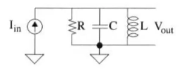
\includegraphics[scale=2]{RisonatoreParallelo.png} 
\centering
\caption{Schema circuitale di un risonatore parallelo}
\label{fig:foo}
\end{figure}
In questa figura è mostrato il risonatore parallelo, l'ammettenza del circuito vale 
$Y=G+j\omega C+\frac{1}{j\omega L}=G+j(\omega C-\frac{1}{\omega L}$ da cui $\omega_0C-\frac{1}{\omega _0L})=0 \Rightarrow \omega _0=\frac{1}{\sqrt{LC}}$ dove $\omega _0$ è la frequenza di risonanza, G è la conduttanza del resistore, gli altri due termini sono le reattanze dei due elementi reattivi.
Alla risonanza le correnti del capacitore e dell'induttore si "annullano" a vicenda,per cui dal generatore viene vista solo la resistenza. 
\subsection{La purezza spettrale}
Facendo un analisi in frequenza della forma d'onda generata da un oscillatore, dovremmo vedere una linea verticale in corrispondenza della frequenza di oscillazione e zero altrove, tuttavia questo non è possibile dal punto di vista pratico, lo spettro di un oscillatore reale mostra che c'è della potenza anche in un intorno più o meno stretto della frequenza centrale.
Questo concetto viene definito rumore di fase.

~\begin{figure}[H]
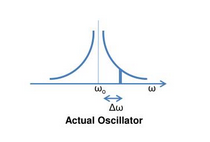
\includegraphics[scale=2]{PhaseNoise.png} 
\centering
\caption{Spettro di un oscillatore reale.}
\label{fig:foo}
\end{figure}

\subsection{Il fattore di merito}
Il concetto di fattore di merito è l'energia immagazzinata all'interno del risonatore, il momento in cui la corrente è nulla nell'induttore corrisponde a quella in cui la tensione sul condensatore è massima, l'energia del condensatore è $\frac{1}{2}CV^2$.

Quando il condensatore si scarica al minimo, la corrente dell'induttore sarà massima, per cui l'energia sarà contenuta nel campo magnetico dell'induttore determinato da $\frac{1}{2}LI^2$.
Il fattore di merito ci dice quanta di questa energia dissipiamo:

$Q=\omega\frac{EnergiaImmagazzinata}{PotenzaMediaDissipataPerPeriodo}$
\centering

Nella configurazione parallelo vista in precedenza $Q=\frac{1}{\sqrt{LC}}\frac{\frac{1}{2}CV^2}{\frac{1}{2}RI^2}=\frac{R}{\sqrt{\frac{L}{C}}}$.

Dalla prima equazione vista, ovvero quella del calcolo di $\omega_0$ partendo da L e C, e sapendo che la richiesta è far oscillare il nostro sistema a 5MHz, è stato deciso di utilizzare (tra le infinite possibilità di valori) C=100pF e L=10uH per via della facile reperibilità di questi componenti.

Con questi valori possiamo calcolarci l'impedenza caratteristica della rete:
$Z_0=\sqrt{\frac{L}{C}}=316\Omega$
\centering

Più il fattore di merito aumenta e più la curva dello spettro sarà "appuntita", il che vuol dire meno rumore di fase, un oscillatore al quarzo di buona qualità ha un fattore di merito Q=10000, un oscillatore a componenti tradizionali potrebbe arrivare a circa Q=5.

Introduciamo un nuovo concetto: la larghezza di banda dello spettro.

In questo caso si intende la banda in cui lo spettro sta dentro il range di -3dB del massimo.
Facendo un semplice calcolo è possibile vedere che il rapporto tra la larghezza di banda e la frequenza centrale è pari a 1/Q.
Ovviamente questo vuol dire che più la banda è stretta maggiore sarà il fattore di merito.
Il problema di questa realizzazione è che bisogna confrontarsi con i limiti del mondo reale, quindi la resistenza non sarà in parallelo a L e C ma la troveremo in serie a L, perché modelliamo l'induttore reale come un induttore ideale con una resistenza serie.
Ipotizziamo che $RL_S$ e $RL_P$ siano equivalenti, supponendo un Q elevato otteniamo che $R_P=R_S*Q^2$  e $L_p=L_s$.
A questo punto, ricordandoci che L=10uH, $\omega_0=2\pi * 5MHz$, la $R_s$ la andiamo a cercare su un datasheet di un induttore reale e troviamo che è circa $1\Omega$, possiamo calcolarci Q che sarà pari a 316 e per quanto detto prima $R_p=R_sQ^2=10k\Omega$.


~\begin{figure}[H]
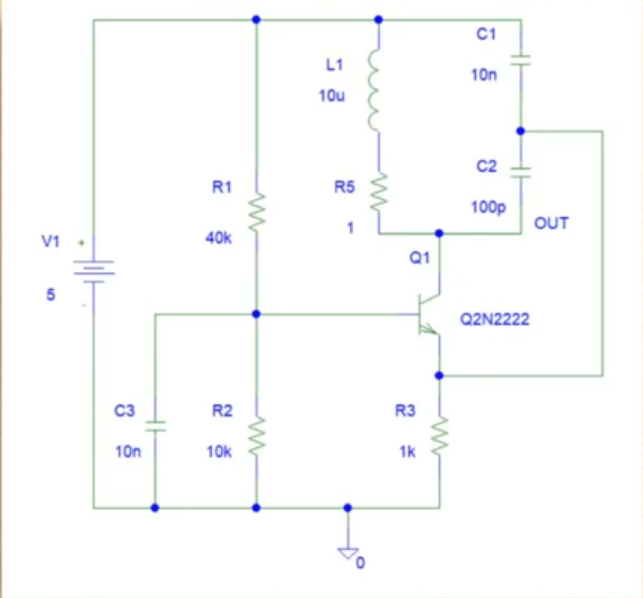
\includegraphics[scale=0.8]{Oscillatore.png}
\centering
\caption{Schema circuitale dell'oscillatore}
\label{fig:foo}
\end{figure}

Questo è il caso in cui Q=316, supponendo che il transistor sia in ZAD, il collettore ha un'impedenza molto elevata, quindi non abbiamo problemi, tuttavia la retroazione tra l'emettitore e il partitore resistivo presenta una impedenza d'ingresso dello stadio a base comune.\\
Qual è l'impedenza vista da quella porta? Andiamo ad analizzare il circuito ai piccoli segnali, ipotizzando che il segnale di ingresso $V_{IN}$ si trovi su $R_3$ con un condensatore di accoppiamento in serie.
~\begin{figure}[H]
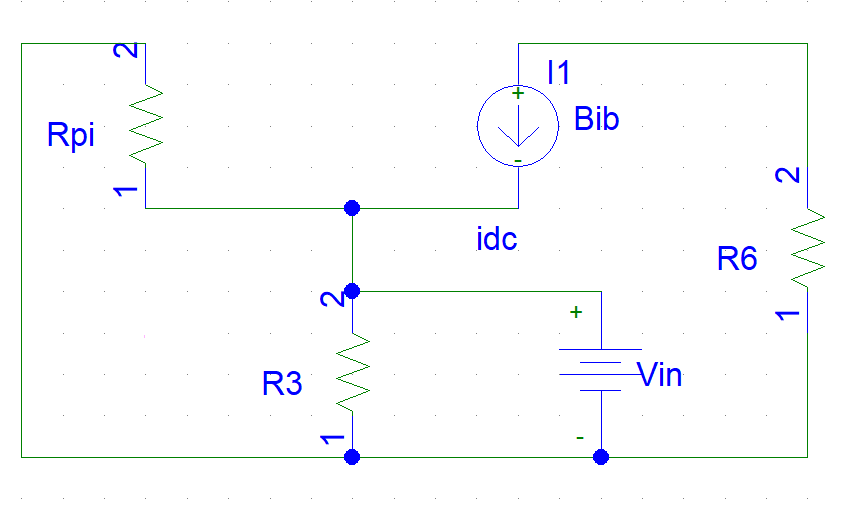
\includegraphics[width=\textwidth]{PiccoliSegnali.png}
\centering
\caption{Circuito ai piccoli segnali}
\label{fig:foo}
\end{figure}
La $ib$ che pilota il generatore di corrente è ovviamente quella che scorre in $r_\pi=\frac{V_T}{I_B}=\frac{0.025}{2.6\mu }=9.6k\Omega$\\
A questo punto possiamo calcolare l'impedenza d'ingresso $Z_{IN}=\frac{V_{IN}}{i_{IN}}$\\
$V_{OUT}=- \beta i_b R_6$\\$V_{IN}=-r \pi i_b$\\
$A_V=\frac{V_{OUT}}{V_{IN}}\approx 100$\\
$i_{IN}=i_3-(\beta +1)i_b=V_{IN}(\frac{1}{R_3}+\frac{\beta +1}{r_\pi})$\\
Andando a sostituire $i_b=-\frac{V_{IN}}{r\pi}$ e $i_3=\frac{V_{IN}}{R_3}$ otteniamo che \\
$Z_{IN}=\frac{1}{\frac{1}{R_3}+\frac{\beta +1}{r_\pi}}\approx 70\Omega$
\paragraph{Prima simulazione del circuito:}
Andando a simulare il risonatore otteniamo quanto segue:
~\begin{figure}[H]
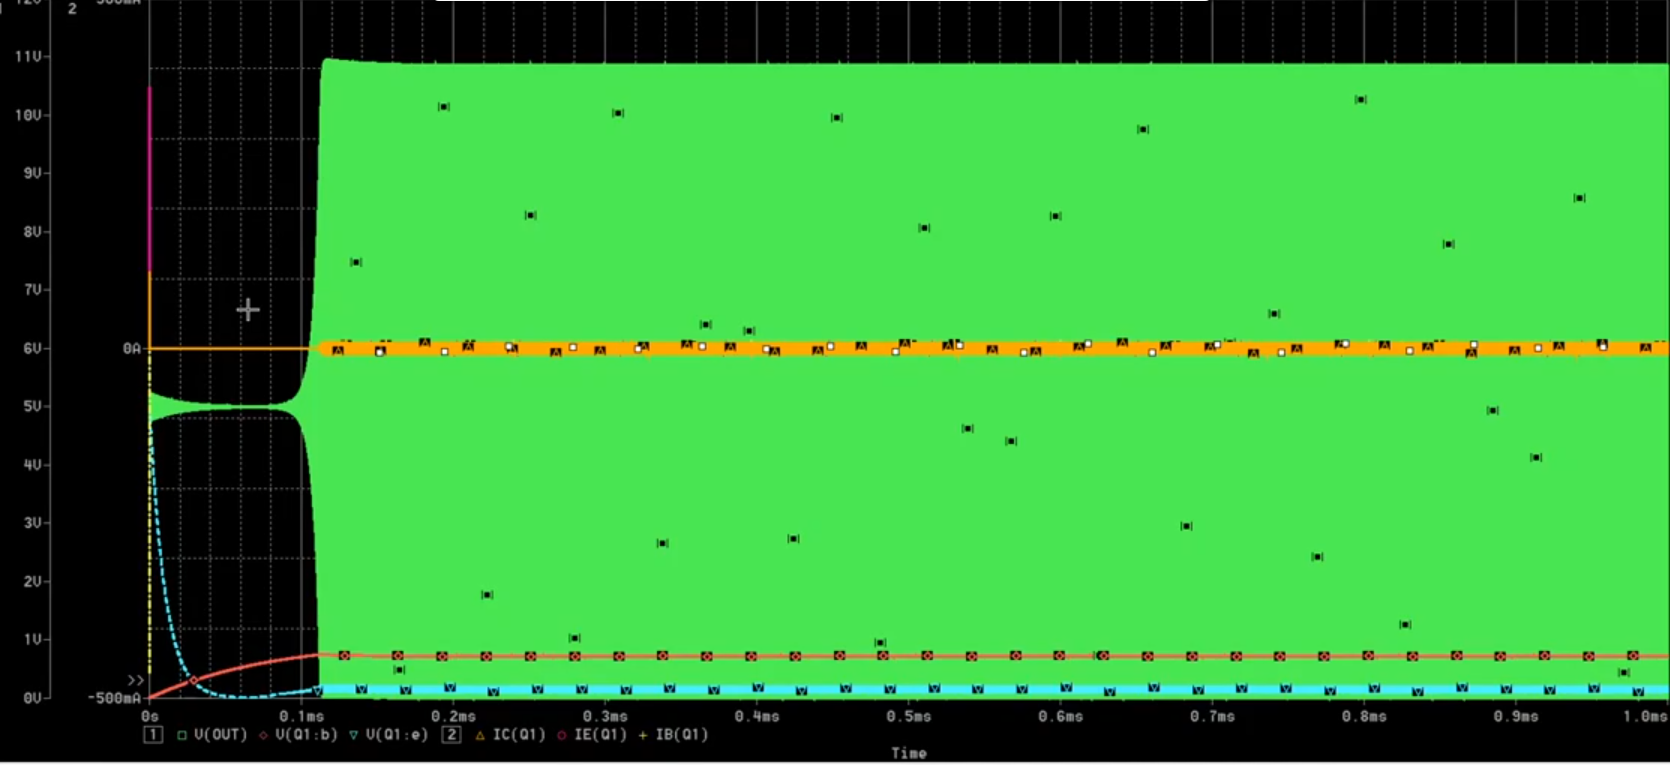
\includegraphics[width=\textwidth]{RisonatoreSimulazione.png}
\centering
\caption{Simulazione nel tempo}
\label{fig:foo}
\end{figure}
Il transistor inizialmente è "spento", la linea rossa è la tensione sulla base, il condensatore C3 inizialmente è scarico, ma grazie ad R1 si carica, quando inizia a superare gli 0.8/0.9 V, fa sì che la corrente in base diventi sufficiente per polarizzare direttamente la giunzione e l'oscillazione possa iniziare.\\la tensione sull'emettitore invece inizialmente è alta perché la tensione ai capi di C1, essendo scarico, è 0V.
Quando la tensione di collettore( rappresentata in verde), tocca la tensione di base( rossa) significa che VCB=0  e quando scende al di sotto perdiamo la polarizzazione in ZAD,infatti  la tensione di collettore presenta un taglio come si può vedere nella figura 6.
~\begin{figure}[H]
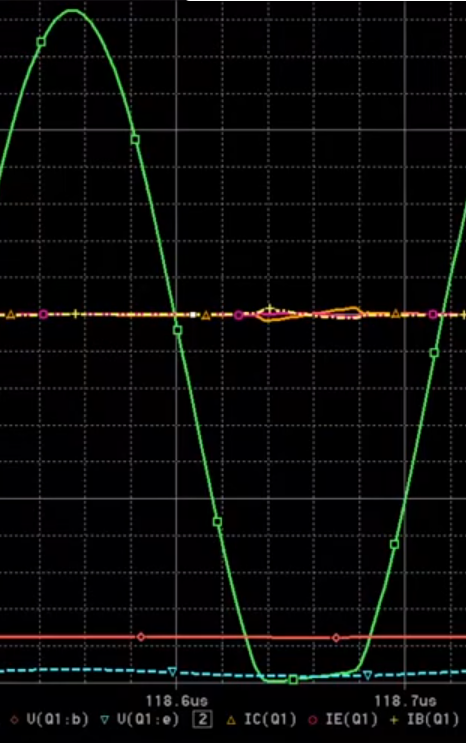
\includegraphics[scale=0.5]{SimulazioneTaglio.png}
\centering
\caption{Taglio dovuto all'uscita del transistor dalla ZAD}
\label{fig:foo}
\end{figure}
Se faccio un'analisi spettrale e calcolo la distorsione armonica totale (THD, ci indica la qualità della forma d'onda d'uscita in relazione alla potenza delle armoniche superiori in confronto all'armonica fondamentale), calcolandola riferita alle prime 4 armoniche, otteniamo un THD del 7.4\%, molto alto!\\
Questa distorsione è dovuta in gran parte al taglio che la sinusoide subisce, quindi dobbiamo aggiungere un controllo automatico dell'ampiezza per evitare che la tensione di collettore scenda al di sotto di quella di base.
Dobbiamo portare il picco massimo intorno agli 8-9V. Per questo scopo utilizziamo un raddrizzatore a singola semionda.
~\begin{figure}[H]
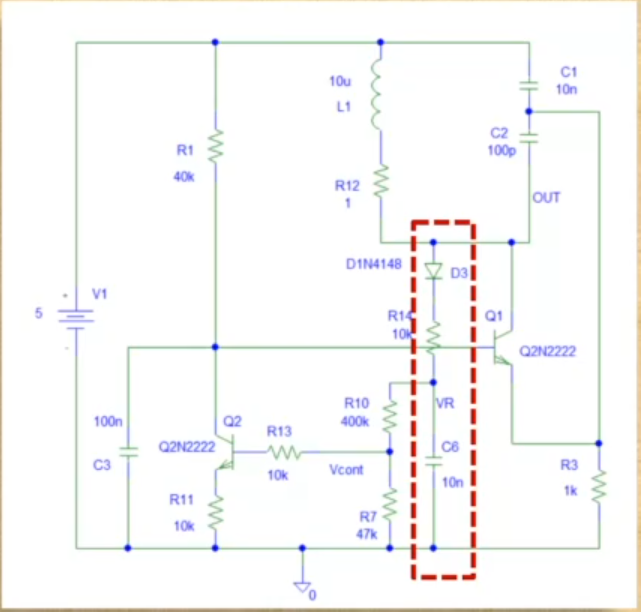
\includegraphics[scale=0.9]{RSS.png}
\centering
\caption{Circuito con il raddrizzatore a singola semionda}
\label{fig:foo}
\end{figure}
In figura 7 i nuovi componenti aggiunti sono riconoscibili dal rettangolo verde \textbf{T2}, formano il circuito rilevatore di massimo, la R serve solamente a caricare meno il risonatore limitando la corrente(in seguito verrà infatti tolta), la tensione $V_R$ sarà quella "raddrizzata" e sarà pari a $V_{MAX}-V\gamma-VR14$, la coppia R10 e R7 funziona solamente da partitore resistivo, Q2 chiude il loop di controllo per portare il guadagno ad anello pari a 1.

Questo porta ad avere un pericolo di instabilità, all'aumentare di VR, Q2 entra in conduzione togliendo corrente alla base di Q1, facendo smettere di oscillare la tensione di collettore.
Devo introdurre un polo dominante e lo ottengo abbassando il condensatore C3 per avere un margine di fase sufficiente per avere un sistema stabile.
Il blocco \textbf{T1} è l'oscillatore (Risonatore, transistor G1 di guadagno, partitore \textbf{P1}), ad ogni ciclo, Q1 aumenta la tensione di elongazione in base alla tensione di base.
Q1, dal punto di vista dell'oscillatore, funziona come amplificatore a base comune per mantenere l'oscillazione, però il guadagno è determinato dalla tensione di base: se la tensione (e corrente) di base aumenta $\Rightarrow$ tensione(e corrente) di collettore aumenta, facendo aumentare la tensione sul diodo D3 che, al mezzo ciclo successivo, fa salire la sinusoide più in alto rispetto a prima.\\
\textbf{T3} è un circuito RC.
I blocchi \textbf{T1,T2,T3} hanno 3 costanti di tempo, infatti quando il diodo D3 è in conduzione possiamo considerarlo come un corto circuito,che collega C6 al risonatore, quando non conduce è un circuito aperto, lasciando C6 "appeso", trovandosi come carico R10 in serie con R7 e la $Z_{IN}$ di Q2(molto elevata).
T1 invece è più complicata da trattare, dato un oscillatore con il suo fattore di merito Q, la costante di tempo dell'inviluppo è pari a $2*R*C$ (The design of CMOS Radio-Frequency integrated Circuits - T.H. Lee).
A questo punto:\\ $T_1=2*R*C=87.5k\Omega *100pF=17.5\mu s \Rightarrow f_1\approx 9kHz$\\
Per quanto detto prima invece:\\ $T_2=RC=\approx 450k\Omega *10nF=4.5ms \rightarrow f2\approx 35Hz$ e\\ $T_3=RC=40k\Omega *100nF=4ms \rightarrow f_3\approx 40Hz$.\\
Se facessimo il diagramma di Bode di questi dati, avremmo la conferma che $f_2$ e  $f_3$ abbiano necessità di essere spostati in avanti per poter avere la stabilità.\\Come procedere adesso?\\
\begin{itemize}
\item $T_2$:$C_6$ lo riduco di 3 ordini di grandezza portandolo a C6=10pF, non ho necessità di una capacità così elevata per "inseguire" l'inviluppo a 5MHz, pertanto mi basta che $T_2>\frac{1}{10}\frac{1}{5MHz}=\frac{1}{10}200ns$, sposto $f_2=35kHz$.
Come detto in precedenza posso rimuovere anche la R che limitava la corrente.
\item Per spostare $T_3$ occorre diminuire C3 a 5nF, portando $f_3=800Hz$
\end{itemize}
Ora abbiamo migliorato la situazione stabilità, ora potremmo diminuire un po' il fattore di guadagno per andare a ricavare più margine di fase.
Possiamo procedere aumentare la capacità C1, abbassando così il guadagno dell'oscillatore.
Un aumento di C1($10nF\Rightarrow 40nF$) mi provoca una partizione di tensione sull'emettitore più bassa, riducendo così il suo guadagno.
A questo punto possiamo alzare il guadagno dello stadio Q2, aumentando la resistenza R11($330\Omega \Rightarrow 1k\Omega$), facendo questa modifica però, modifico anche la tensione di controllo che mi porta ad avere un aumento significativo dell'ampiezza massima della sinusoide in uscita.
Ricordando che la resistenza R7 determina la partizione di VR che portiamo alla base di Q2, possiamo modificarla per abbassare la tensione di controllo $V_{CONT} \approx V_R*\frac{R_7}{R_7+R_10}$.
Dobbiamo tenere conto che andando a modificare R7 andrò anche a peggiorare il fattore distorsione della forma d'onda.
Svolgendo una serie di prove possiamo disegnare un grafico:
~\begin{figure}[H]
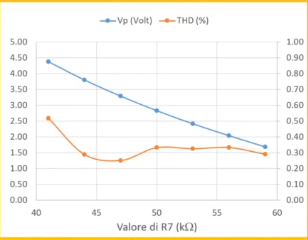
\includegraphics[width=\textwidth]{SceltaR7.png}
\centering
\caption{Scelta di R7}
\label{fig:foo}
\end{figure}
In arancione abbiamo la distorsione, in blu la tensione di picco che va dai 4.5V(caso molto limite) agli 1.75V.

Posso prendere il valore di $50k\Omega$ così da ottenere, come si può vedere dal grafico, un THD del 3\% ed una tensione di picco intorno ai 3V, non rischiando di uscire fuori dalla tensione massima. 

A questo punto ottengo un risultato accettabile:
~\begin{figure}[H]
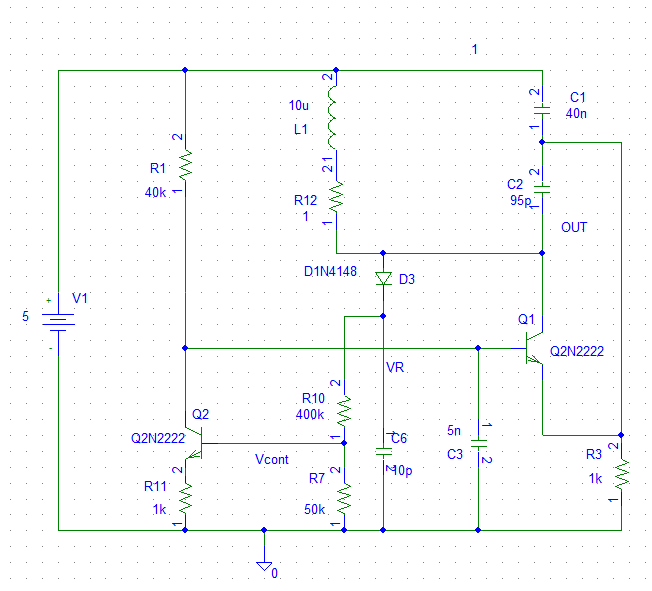
\includegraphics[width=\textwidth]{NuovoSchema.png}
\centering
\caption{Schema circuitale con i nuovi valori}
\label{fig:foo}
\end{figure}

~\begin{figure}[H]
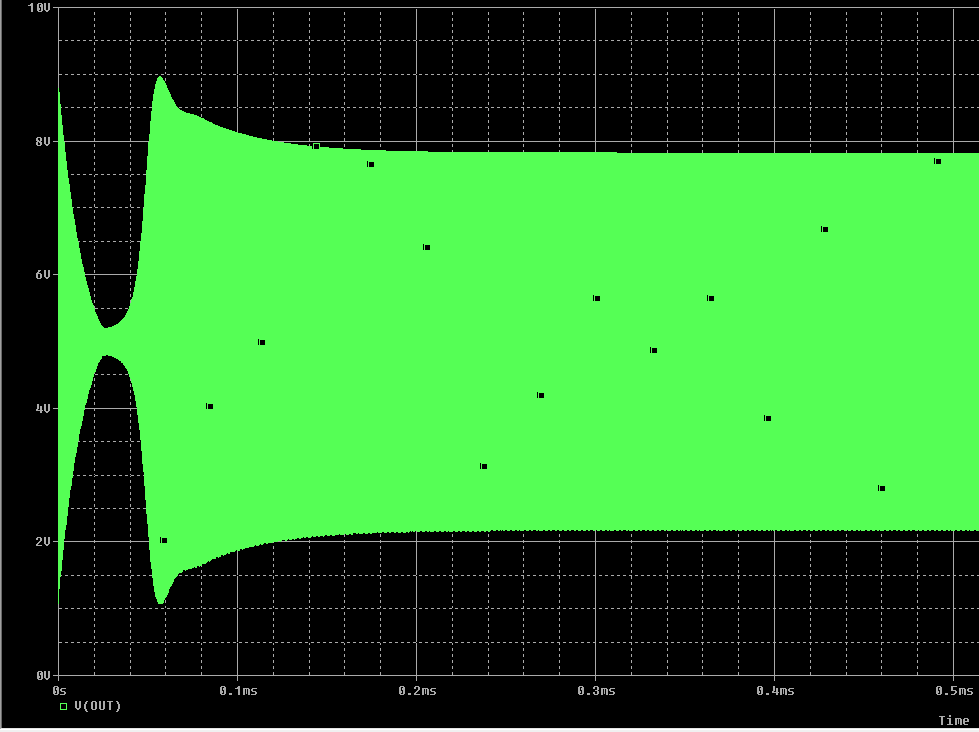
\includegraphics[width=\textwidth]{SimulazioneNuova.png}
\centering
\caption{Risultato della simulazione nel tempo}
\label{fig:foo}
\end{figure}
Dopo il primo transitorio e quando la tensione sulla base è sufficiente per innescare l'oscillazione, questa viene limitata dalla non linearità del transistor, in seguito, quando il loop di controllo  si attiva, la tensione di oscillazione diminuisce e arrivo al risultato desiderato, infatti facendo uno zoom sull'onda che ottengo dopo il tempo necessario al circuito per limitare la tensione di oscillazione:
~\begin{figure}[H]
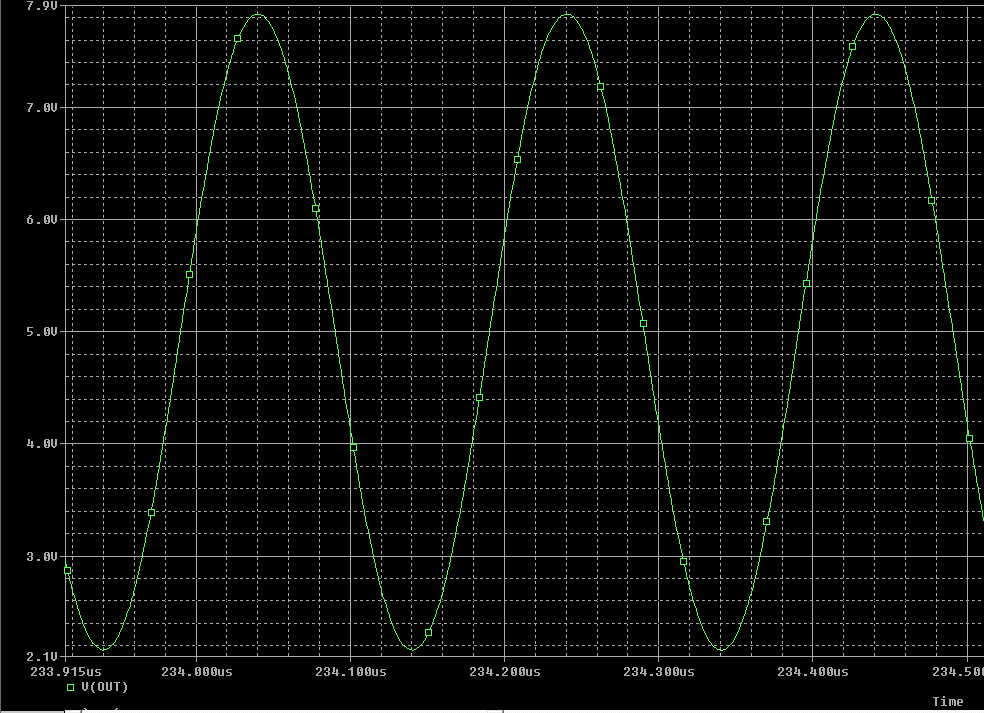
\includegraphics[width=\textwidth]{SimulazioneNuovaZoom.png}
\centering
\caption{Zoom sulla forma d'onda}
\label{fig:foo}
\end{figure}

A questo punto dovremmo tenere conto del fatto che il diodo in regime dinamico introduce una capacità in funzione della sua polarizzazione inversa.\\
Sapendo che:\\  \LARGE$\bm{Z_C=\frac{1}{j \omega C}=\frac{V}{I} \rightarrow C=\frac{\bar{I}}{\omega \bar{V}}}$ \normalsize possiamo simulare in frequenza come si comporta un diodo(nel nostro caso abbiamo simulato un D1N4148 $https://www.vishay.com/docs/81857/1n4148.pdf$)
~\begin{figure}[H]
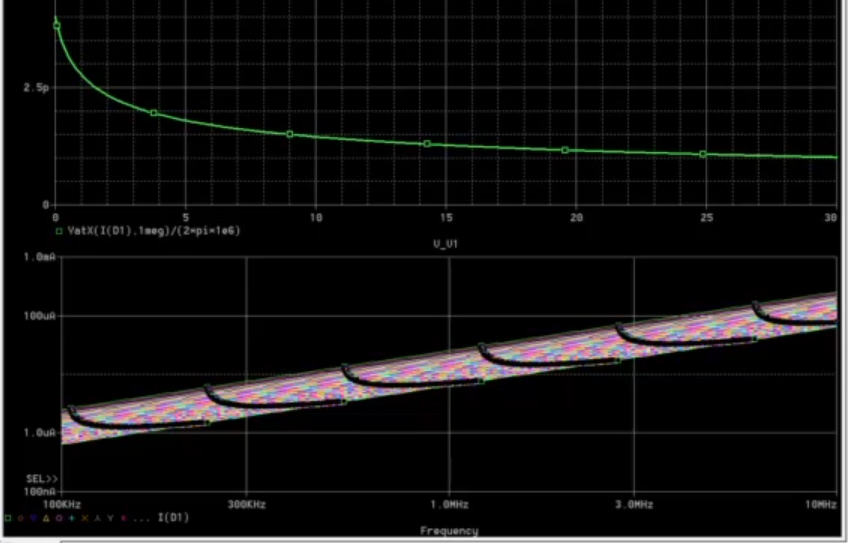
\includegraphics[width=\textwidth]{D1N4148.png}
\centering
\caption{Simulazione in frequenza del comportamento di un D1N4148}
\label{fig:foo}
\end{figure}
Nel grafico sotto possiamo vedere la corrente in funzione della frequenza, come ci aspettavamo possiamo vedere che la corrente sale all'aumentare della frequenza $\rightarrow$ effetto capacitivo.\\Nel grafico sopra vediamo l'effetto capacitivo del diodo ad 1MHz.
A questo punto potremmo simulare anche il comportamento del diodo scelto per il nostro oscillatore per introdurre una capacità variabile:  Il varactor BBY58 ($https://www.infineon.com/dgdl/Infineon-BBY58SERIES-DS-v01_01-en.pdf?fileId=5546d4624933b8750149880de2927e14$) dal datasheet: 
~\begin{figure}[H]
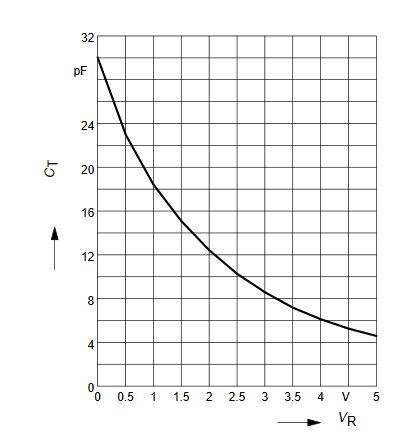
\includegraphics[width=\textwidth]{BBY58.png}
\centering
\caption{Effetto capacitivo del BBY58}
\label{fig:foo}
\end{figure}
Alla luce di questi nuovi punti, possiamo andare a modificare ed ultimare il nostro oscillatore come segue:
~\begin{figure}[H]
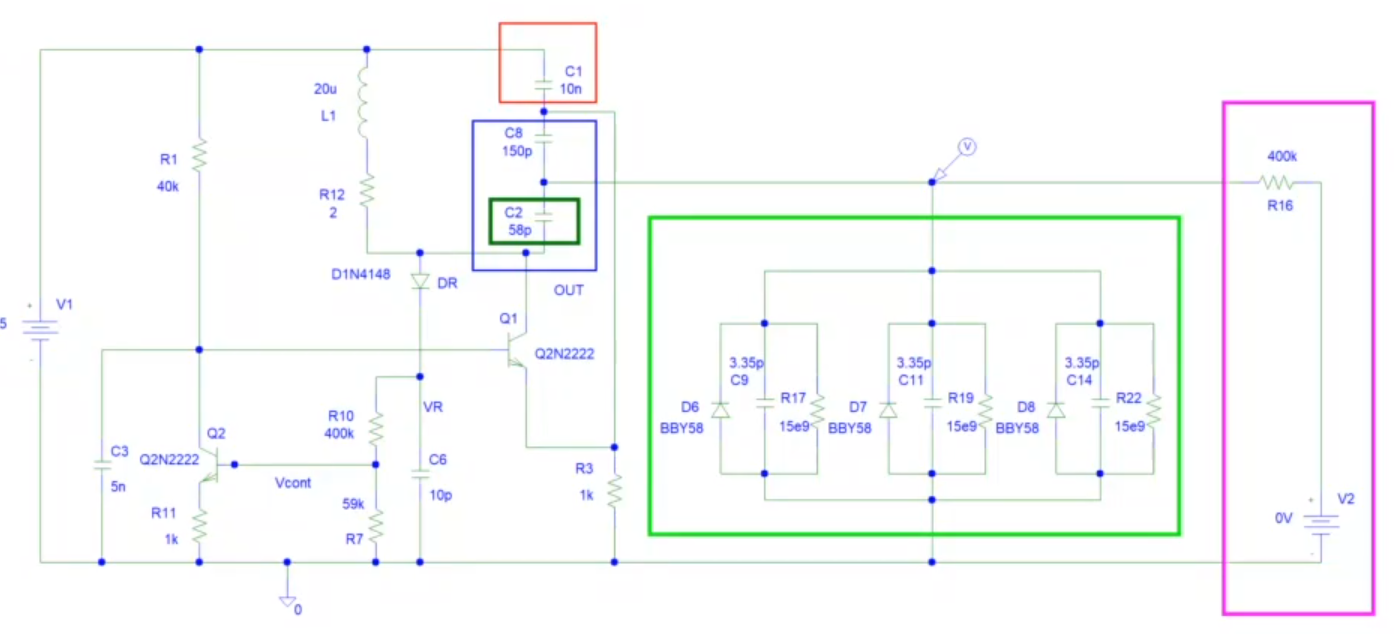
\includegraphics[width=\textwidth]{UltimoOscillatore.png}
\centering
\caption{Realizzazione finale dell'oscillatore}
\label{fig:foo}
\end{figure}
Nel blocco verde chiaro notiamo che ci sono 3 blocchetti in parallelo per cercare di avere una capacità un po' più grande e poter quindi agire sulle frequenze che ci interessano, considerando che le specifiche ci richiedono una banda di sintonia pari al 2\%(100kHz) della frequenza di oscillazione.
Anche alla polarizzazione massima ho comunque una capacità di almeno 10pF dovuti  a C9, C11 e C14 che presentano una capacità costante.
Abbiamo creato una rete di polarizzazione, rettangolo fucsia, la R è elevata per non influire sul Q del risonatore.
Abbiamo inserito una capacità di sintonia(rettangolo blu), divisa in due in modo tale che quel nodo non influenzi il circuito.
La C2 in precedenza era 100pF, dividendola in due avremmo ottenuto 50pF, tuttavia per mantenere costante la frequenza è stato necessario raddoppiare l'induttanza(20uH) che provoca un aumento della resistenza serie.
Il rapporto \LARGE$\bm{\frac{L}{R_s}}$ \normalsize determina il Q e la resistenza parallelo equivalente dipende da $Q^2$.
Se non avessi raddoppiato $R_s=R12$, avrei avuto un $R_p$ quadruplicata, con una conseguente rischio di instabilità.
Per risolvere questo problema sono state inserite quindi C8 e C2 pari rispettivamente a 150pF e 58pF per fare in modo che la tensione sui varactor sia abbastanza bassa da non farli polarizzare direttamente, dato che la loro peculiarità di introdurre una capacità nel circuito è data dalla polarizzazione inversa.\\Dalla figura 13 vediamo che il varactor introduce, nel range $1V \div 5V$ una capacità $18pF \div 5pF$, avendone 3 in parallelo avremo un intervallo che va dai 54pF ai 15pF, ricordando inoltre le 3 capacità fisse abbiamo un intervallo $25pF \div 64pF$.
A questo punto possiamo simulare su PSpice il circuito così ottenuto(figura 14), parametrizzando la tensione di controllo da 1 a 5V ed otteniamo:
~\begin{figure}[H]
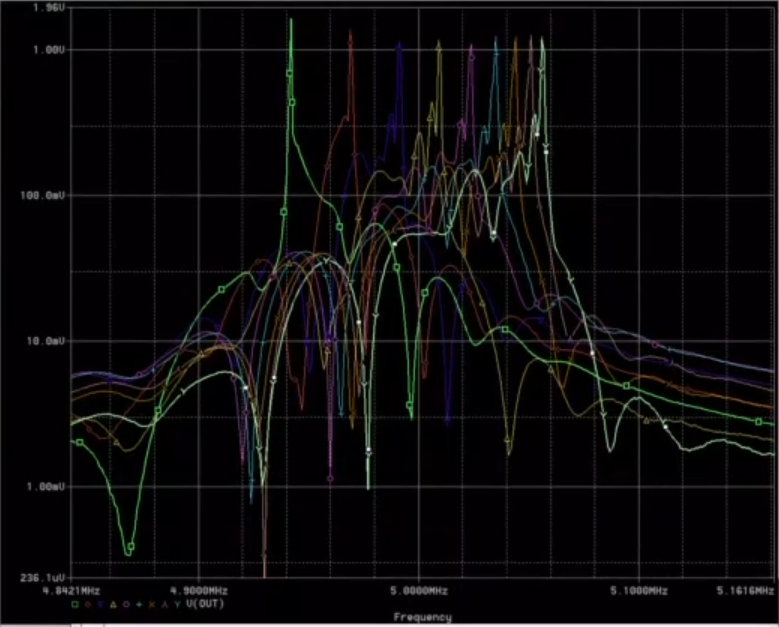
\includegraphics[width=\textwidth]{AnalisiSpettraleFinale.png}
\centering
\caption{Analisi Spettrale dell'oscillatore}
\label{fig:foo}
\end{figure}
Sotto 1V non possiamo scendere per evitare di polarizzare direttamente i varactor, che porterebbe un abbassamento del fattore Q ed una distorsione causato dal carico non simmetrico sulle due semionde.\\Possiamo procedere alla simulazione anche su LTSpice($https://www.analog.com/en/design-center/design-tools-and-calculators/ltspice-simulator.html$), il circuito è il medesimo di prima e possiamo andare a leggere la Total Harmonic Distorsion del nostro oscillatore:
~\begin{figure}[H]
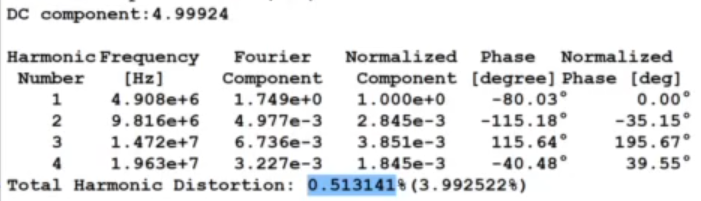
\includegraphics[width=\textwidth]{THDLT.png}
\centering
\caption{THD calcolata da LTSpice}
\label{fig:foo}
\end{figure}
Possiamo vedere una THD più che accettabile, pari al 0.51\%.
Ci rimane da progettare uno stadio d'uscita per non influenzare eccessivamente il fattore Q dell'oscillatore, dobbiamo cercare un operazionale abbastanza veloce(slew-rate).
$V_{OUT}=V_m * \sin(\omega t) $\\$\frac{dV_{OUT}}{dt}=\omega V_m \cos(\omega t)$\\$V_m=2V$ da specifica(vorrei una tensione di 1V sul carico, e stiamo ipotizzando una resistenza di carico $R_L$ pari a $50\Omega$ e una impedenza interna pari anch'essa a $50\Omega$).
La pendenza massima di una sinusoide ce l'ho all'intersezione con l'asse orizzontale, infatti la sua derivata è il coseno ed in quel punto vale 1.
La pendenza massima quindi è pari a $2 \pi f V_m=4\pi * 5 *10^6=63*10^6=63\frac{V}{\mu s}$.
A questo punto è possibile andare sul sito di un qualsiasi rivenditore di componenti e scegliere un amplificatore operazionale che rispetti questa caratteristica, nel nostro caso abbiamo usato $www.digikey.it$, filtrando in base allo slew-rate,all'impedenza d'ingresso alta, per evitare di influenzare il resto del circuito $\rightarrow$ corrente di polarizzazione bassa, larghezza di banda minima possiamo scegliere 100MHz, abbiamo tutti che soddisfano le nostre esigenze, ad esempio AD8091($https://www.analog.com/media/en/technical-documentation/data-sheets/AD8091_8092.pdf$).
~\begin{figure}[H]
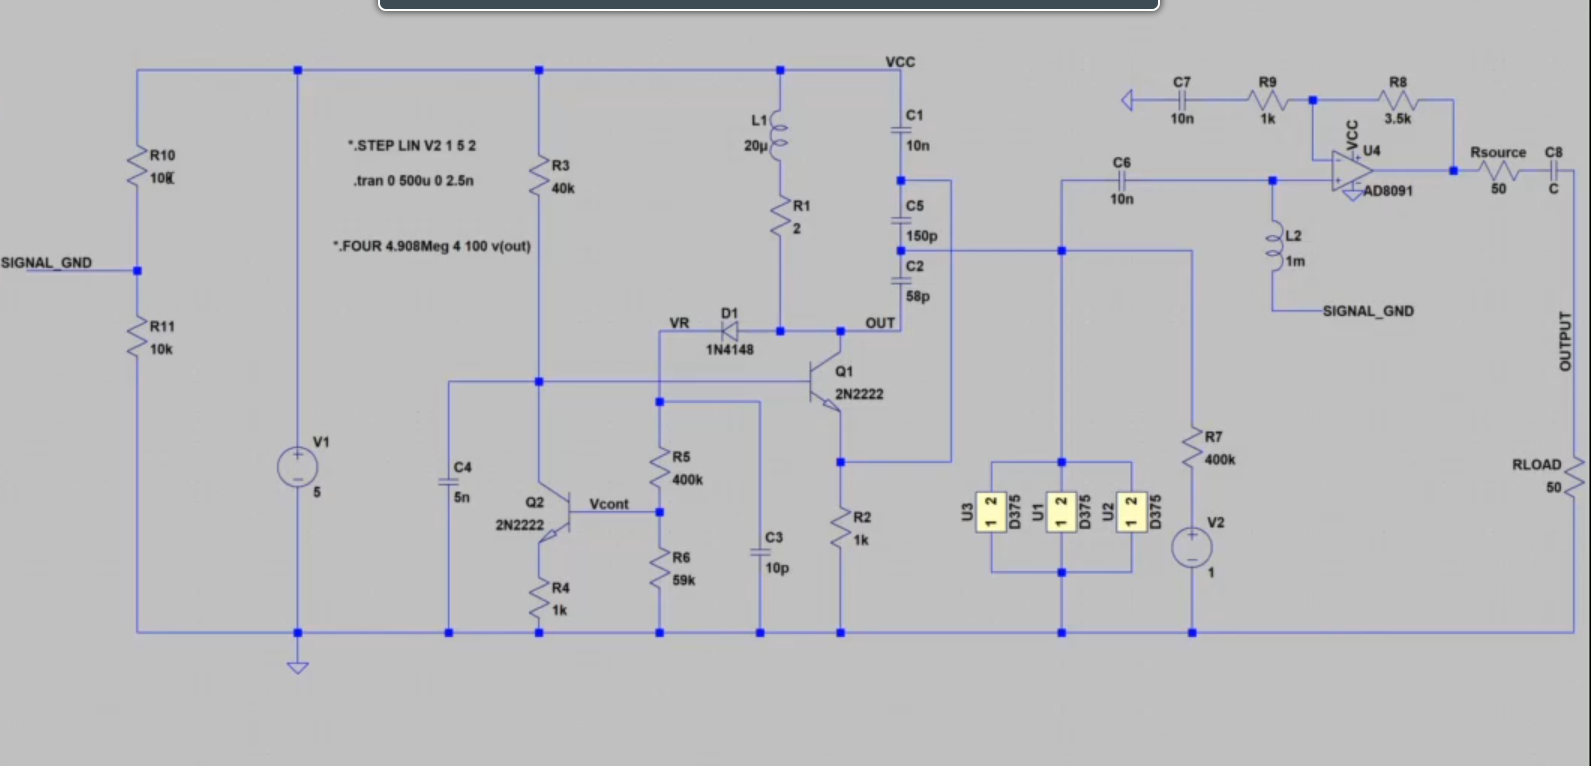
\includegraphics[width=\textwidth]{CircuitoConBuffer}
\centering
\caption{Circuito con lo stadio di uscita}
\label{fig:foo}
\end{figure}

%%%%Devo concludere con 1:57 ultimo video
\newpage
\section{Realizzazione}

\newpage
\section{Risultati}

\newpage

\section{Conclusioni}

\newpage
\section{Riferimenti}

\begin{itemize}
\item The Design of CMOS Radio-Frequency Integrated Circuits - Thomas H. Lee
\item RF Microeletronics - B. Razavi
\item D1N4148 - $https://www.vishay.com/docs/81857/1n4148.pdf$
\item PSpice
\item LTSpice - $https://www.analog.com/en/design-center/design-tools-and-calculators/ltspice-simulator.html$
\item $https://www.analog.com/media/en/technical-documentation/data-sheets/AD8091_8092.pdf$
\item $www.digikey.it$
\end{itemize}
\end{document}
